\chapter{Modelling}

% Data Flow Diagram
% State Transition Diagram

\section{Data Flow Diagram}

\begin{figure}[h]
	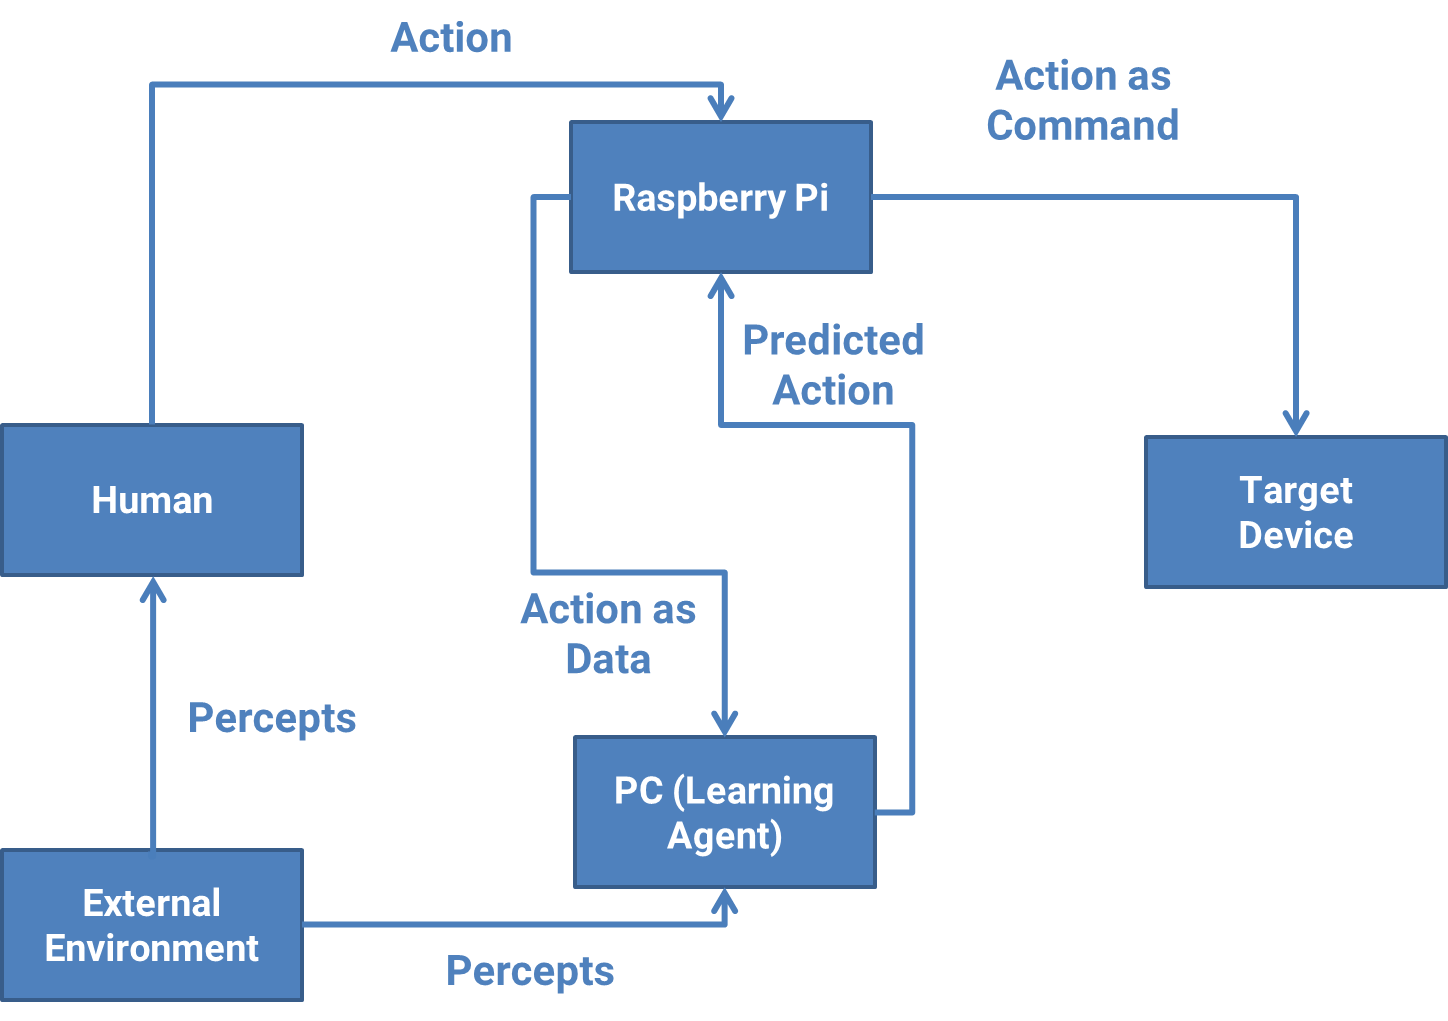
\includegraphics[width=\textwidth]{./Chapter4/dfd}
		\caption{Data Flow Diagram}
\end{figure}

\section{State Transition Diagram}

\begin{figure}[h]
	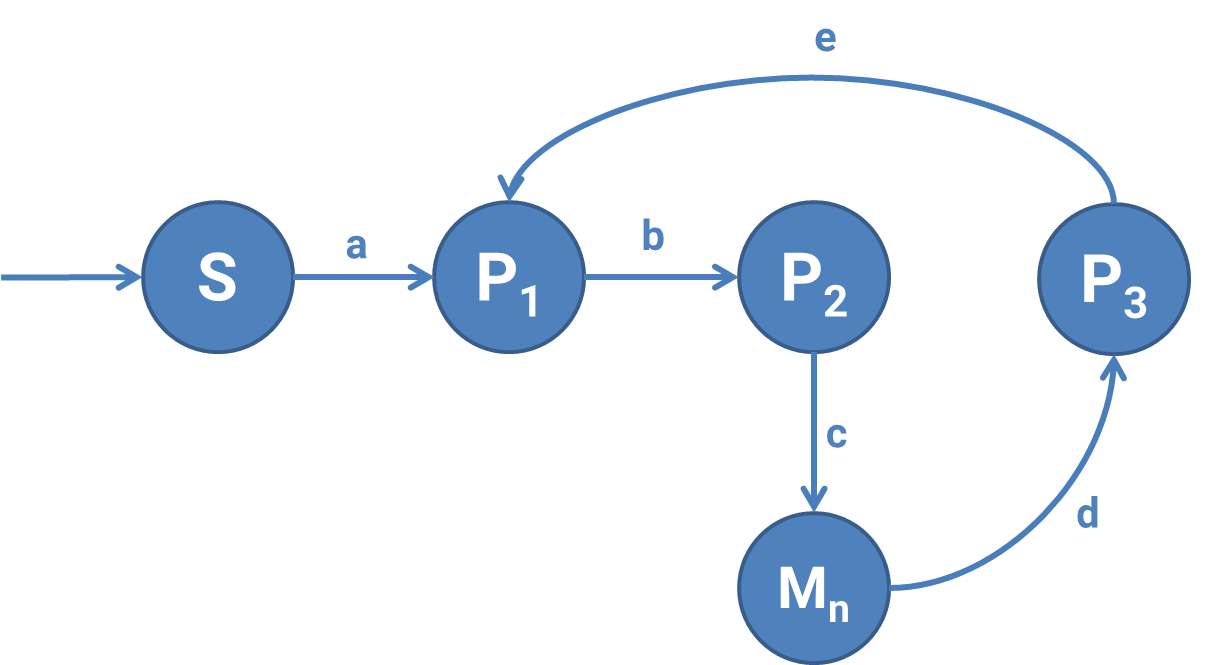
\includegraphics[width=\textwidth]{./Chapter4/state-transition}
		\caption{State Transition Diagram}
\end{figure}

Where,\\
\hspace*{1cm} S: Start state\\
\hspace*{1cm}P1: Phase 1- Observation and collection of usage data.\\
\hspace*{1cm}P2: Phase 2- Run machine learning algorithms on collected data to generate a prediction model.\\
\hspace*{1cm}Mn: Prediction Model- Current (nth) prediction model. n is the total number of discrete anomalies detected since start.\\
\hspace*{1cm}P3: Phase 3- Detect anomalies and modify data collected in Phase 1 to match the anomalies.\\\\
\hspace*{1cm}a: Create a mutable table for holding observed data for the learning agent to process.\\
\hspace*{1cm}b: Data collection threshold reached or data modification completed.\\
\hspace*{1cm}c: Prediction Model generated.\\
\hspace*{1cm}d: Anomaly detected. This implies change in user habit or detection of a new habit.\\
\hspace*{1cm}e: Make corrections in the table to avoid anomalies in the near future.\\

\paragraph{}
Our system does not have any state of absolute success. Success and failure are both temporary and the system is designed to learn from its mis-predictions. The canonical success in this project will be the usability of the machine learning system. The more data it is exposed to, the more successful the prediction model will be.

\begin{comment}
\begin{figure}
	\includegraphics[width=\textwidth]{Flower}
		\caption{A Flower}
\end{figure}
\end{comment}